\documentclass[1p]{elsarticle_modified}
%\bibliographystyle{elsarticle-num}

%\usepackage[colorlinks]{hyperref}
%\usepackage{abbrmath_seonhwa} %\Abb, \Ascr, \Acal ,\Abf, \Afrak
\usepackage{amsfonts}
\usepackage{amssymb}
\usepackage{amsmath}
\usepackage{amsthm}
\usepackage{scalefnt}
\usepackage{amsbsy}
\usepackage{kotex}
\usepackage{caption}
\usepackage{subfig}
\usepackage{color}
\usepackage{graphicx}
\usepackage{xcolor} %% white, black, red, green, blue, cyan, magenta, yellow
\usepackage{float}
\usepackage{setspace}
\usepackage{hyperref}

\usepackage{tikz}
\usetikzlibrary{arrows}

\usepackage{multirow}
\usepackage{array} % fixed length table
\usepackage{hhline}

%%%%%%%%%%%%%%%%%%%%%
\makeatletter
\renewcommand*\env@matrix[1][\arraystretch]{%
	\edef\arraystretch{#1}%
	\hskip -\arraycolsep
	\let\@ifnextchar\new@ifnextchar
	\array{*\c@MaxMatrixCols c}}
\makeatother %https://tex.stackexchange.com/questions/14071/how-can-i-increase-the-line-spacing-in-a-matrix
%%%%%%%%%%%%%%%

\usepackage[normalem]{ulem}

\newcommand{\msout}[1]{\ifmmode\text{\sout{\ensuremath{#1}}}\else\sout{#1}\fi}
%SOURCE: \msout is \stkout macro in https://tex.stackexchange.com/questions/20609/strikeout-in-math-mode

\newcommand{\cancel}[1]{
	\ifmmode
	{\color{red}\msout{#1}}
	\else
	{\color{red}\sout{#1}}
	\fi
}

\newcommand{\add}[1]{
	{\color{blue}\uwave{#1}}
}

\newcommand{\replace}[2]{
	\ifmmode
	{\color{red}\msout{#1}}{\color{blue}\uwave{#2}}
	\else
	{\color{red}\sout{#1}}{\color{blue}\uwave{#2}}
	\fi
}

\newcommand{\Sol}{\mathcal{S}} %segment
\newcommand{\D}{D} %diagram
\newcommand{\A}{\mathcal{A}} %arc


%%%%%%%%%%%%%%%%%%%%%%%%%%%%%5 test

\def\sl{\operatorname{\textup{SL}}(2,\Cbb)}
\def\psl{\operatorname{\textup{PSL}}(2,\Cbb)}
\def\quan{\mkern 1mu \triangleright \mkern 1mu}

\theoremstyle{definition}
\newtheorem{thm}{Theorem}[section]
\newtheorem{prop}[thm]{Proposition}
\newtheorem{lem}[thm]{Lemma}
\newtheorem{ques}[thm]{Question}
\newtheorem{cor}[thm]{Corollary}
\newtheorem{defn}[thm]{Definition}
\newtheorem{exam}[thm]{Example}
\newtheorem{rmk}[thm]{Remark}
\newtheorem{alg}[thm]{Algorithm}

\newcommand{\I}{\sqrt{-1}}
\begin{document}

%\begin{frontmatter}
%
%\title{Boundary parabolic representations of knots up to 8 crossings}
%
%%% Group authors per affiliation:
%\author{Yunhi Cho} 
%\address{Department of Mathematics, University of Seoul, Seoul, Korea}
%\ead{yhcho@uos.ac.kr}
%
%
%\author{Seonhwa Kim} %\fnref{s_kim}}
%\address{Center for Geometry and Physics, Institute for Basic Science, Pohang, 37673, Korea}
%\ead{ryeona17@ibs.re.kr}
%
%\author{Hyuk Kim}
%\address{Department of Mathematical Sciences, Seoul National University, Seoul 08826, Korea}
%\ead{hyukkim@snu.ac.kr}
%
%\author{Seokbeom Yoon}
%\address{Department of Mathematical Sciences, Seoul National University, Seoul, 08826,  Korea}
%\ead{sbyoon15@snu.ac.kr}
%
%\begin{abstract}
%We find all boundary parabolic representation of knots up to 8 crossings.
%
%\end{abstract}
%\begin{keyword}
%    \MSC[2010] 57M25 
%\end{keyword}
%
%\end{frontmatter}

%\linenumbers
%\tableofcontents
%
\newcommand\colored[1]{\textcolor{white}{\rule[-0.35ex]{0.8em}{1.4ex}}\kern-0.8em\color{red} #1}%
%\newcommand\colored[1]{\textcolor{white}{ #1}\kern-2.17ex	\textcolor{white}{ #1}\kern-1.81ex	\textcolor{white}{ #1}\kern-2.15ex\color{red}#1	}

{\Large $\underline{11a_{103}~(K11a_{103})}$}

\setlength{\tabcolsep}{10pt}
\renewcommand{\arraystretch}{1.6}
\vspace{1cm}\begin{tabular}{m{100pt}>{\centering\arraybackslash}m{274pt}}
\multirow{5}{120pt}{
	\centering
	\includegraphics[width=112pt]{../../../GIT/diagram.site/Diagrams/png/352_11a_103.png}\\
\ \ \ A knot diagram\footnotemark}&
\allowdisplaybreaks
\textbf{Linearized knot diagam} \\
\cline{2-2}
 &
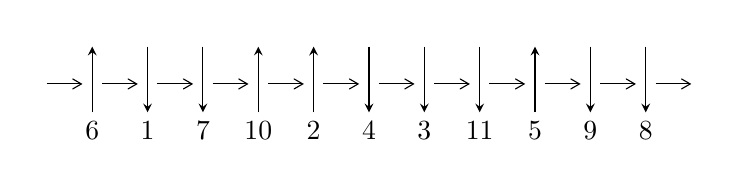
\begin{tikzpicture}[x=20pt, y=17pt]
	% nodes
	\node (C0) at (0, 0) {};
	\node (C1) at (1, 0) {};
	\node (C1U) at (1, +1) {};
	\node (C1D) at (1, -1) {6};

	\node (C2) at (2, 0) {};
	\node (C2U) at (2, +1) {};
	\node (C2D) at (2, -1) {1};

	\node (C3) at (3, 0) {};
	\node (C3U) at (3, +1) {};
	\node (C3D) at (3, -1) {7};

	\node (C4) at (4, 0) {};
	\node (C4U) at (4, +1) {};
	\node (C4D) at (4, -1) {10};

	\node (C5) at (5, 0) {};
	\node (C5U) at (5, +1) {};
	\node (C5D) at (5, -1) {2};

	\node (C6) at (6, 0) {};
	\node (C6U) at (6, +1) {};
	\node (C6D) at (6, -1) {4};

	\node (C7) at (7, 0) {};
	\node (C7U) at (7, +1) {};
	\node (C7D) at (7, -1) {3};

	\node (C8) at (8, 0) {};
	\node (C8U) at (8, +1) {};
	\node (C8D) at (8, -1) {11};

	\node (C9) at (9, 0) {};
	\node (C9U) at (9, +1) {};
	\node (C9D) at (9, -1) {5};

	\node (C10) at (10, 0) {};
	\node (C10U) at (10, +1) {};
	\node (C10D) at (10, -1) {9};

	\node (C11) at (11, 0) {};
	\node (C11U) at (11, +1) {};
	\node (C11D) at (11, -1) {8};
	\node (C12) at (12, 0) {};

	% arrows
	\draw[->,>={angle 60}]
	(C0) edge (C1) (C1) edge (C2) (C2) edge (C3) (C3) edge (C4) (C4) edge (C5) (C5) edge (C6) (C6) edge (C7) (C7) edge (C8) (C8) edge (C9) (C9) edge (C10) (C10) edge (C11) (C11) edge (C12) ;	\draw[->,>=stealth]
	(C1D) edge (C1U) (C2U) edge (C2D) (C3U) edge (C3D) (C4D) edge (C4U) (C5D) edge (C5U) (C6U) edge (C6D) (C7U) edge (C7D) (C8U) edge (C8D) (C9D) edge (C9U) (C10U) edge (C10D) (C11U) edge (C11D) ;
	\end{tikzpicture} \\
\hhline{~~} \\& 
\textbf{Solving Sequence} \\ \cline{2-2} 
 &
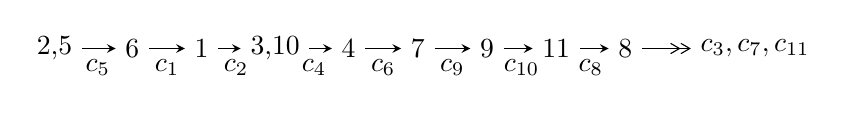
\begin{tikzpicture}[x=25pt, y=7pt]
	% node
	\node (A0) at (-1/8, 0) {2,5};
	\node (A1) at (1, 0) {6};
	\node (A2) at (2, 0) {1};
	\node (A3) at (49/16, 0) {3,10};
	\node (A4) at (33/8, 0) {4};
	\node (A5) at (41/8, 0) {7};
	\node (A6) at (49/8, 0) {9};
	\node (A7) at (57/8, 0) {11};
	\node (A8) at (65/8, 0) {8};
	\node (C1) at (1/2, -1) {$c_{5}$};
	\node (C2) at (3/2, -1) {$c_{1}$};
	\node (C3) at (5/2, -1) {$c_{2}$};
	\node (C4) at (29/8, -1) {$c_{4}$};
	\node (C5) at (37/8, -1) {$c_{6}$};
	\node (C6) at (45/8, -1) {$c_{9}$};
	\node (C7) at (53/8, -1) {$c_{10}$};
	\node (C8) at (61/8, -1) {$c_{8}$};
	\node (A9) at (10, 0) {$c_{3},c_{7},c_{11}$};

	% edge
	\draw[->,>=stealth]	
	(A0) edge (A1) (A1) edge (A2) (A2) edge (A3) (A3) edge (A4) (A4) edge (A5) (A5) edge (A6) (A6) edge (A7) (A7) edge (A8) ;
	\draw[->>,>={angle 60}]	
	(A8) edge (A9);
\end{tikzpicture} \\ 

\end{tabular} \\

\footnotetext{
The image of knot diagram is generated by the software ``\textbf{Draw programme}" developed by Andrew Bartholomew(\url{http://www.layer8.co.uk/maths/draw/index.htm\#Running-draw}), where we modified some parts for our purpose(\url{https://github.com/CATsTAILs/LinksPainter}).
}\phantom \\ \newline 
\centering \textbf{Ideals for irreducible components\footnotemark of $X_{\text{par}}$} 
 
\begin{align*}
I^u_{1}&=\langle 
3278045625361 u^{33}-962912057641220 u^{32}+\cdots+5173973686763240 b-10139327463448051,\\
\phantom{I^u_{1}}&\phantom{= \langle  }165318083439065 u^{33}-292527248838037 u^{32}+\cdots+517397368676324 a-3832627237028687,\\
\phantom{I^u_{1}}&\phantom{= \langle  }u^{34}- u^{33}+\cdots-8 u+1\rangle \\
I^u_{2}&=\langle 
u^9+3 u^7+u^6+3 u^5+2 u^4+3 u^3+u^2+b+2 u+1,\\
\phantom{I^u_{2}}&\phantom{= \langle  }u^{10}+u^9+3 u^8+3 u^7+3 u^6+3 u^5+3 u^4+3 u^3+2 u^2+a+2 u,\\
\phantom{I^u_{2}}&\phantom{= \langle  }u^{12}+4 u^{10}+u^9+6 u^8+3 u^7+7 u^6+3 u^5+7 u^4+3 u^3+3 u^2+2 u+1\rangle \\
I^u_{3}&=\langle 
3 a^2 u-5 a^2- a u+17 b-4 a-14 u-22,\;a^3- a^2 u+5 a u+3 a- u+6,\;u^2+1\rangle \\
\\
\end{align*}
\raggedright * 3 irreducible components of $\dim_{\mathbb{C}}=0$, with total 52 representations.\\
\footnotetext{All coefficients of polynomials are rational numbers. But the coefficients are sometimes approximated in decimal forms when there is not enough margin.}
\newpage
\renewcommand{\arraystretch}{1}
\centering \section*{I. $I^u_{1}= \langle 3.28\times10^{12} u^{33}-9.63\times10^{14} u^{32}+\cdots+5.17\times10^{15} b-1.01\times10^{16},\;1.65\times10^{14} u^{33}-2.93\times10^{14} u^{32}+\cdots+5.17\times10^{14} a-3.83\times10^{15},\;u^{34}- u^{33}+\cdots-8 u+1 \rangle$}
\flushleft \textbf{(i) Arc colorings}\\
\begin{tabular}{m{7pt} m{180pt} m{7pt} m{180pt} }
\flushright $a_{2}=$&$\begin{pmatrix}0\\u\end{pmatrix}$ \\
\flushright $a_{5}=$&$\begin{pmatrix}1\\0\end{pmatrix}$ \\
\flushright $a_{6}=$&$\begin{pmatrix}1\\- u^2\end{pmatrix}$ \\
\flushright $a_{1}=$&$\begin{pmatrix}- u\\u^3+u\end{pmatrix}$ \\
\flushright $a_{3}=$&$\begin{pmatrix}- u^3\\u^5+u^3+u\end{pmatrix}$ \\
\flushright $a_{10}=$&$\begin{pmatrix}-0.319519 u^{33}+0.565382 u^{32}+\cdots-24.1768 u+7.40751\\-0.000633564 u^{33}+0.186107 u^{32}+\cdots-10.0234 u+1.95968\end{pmatrix}$ \\
\flushright $a_{4}=$&$\begin{pmatrix}-1.45002 u^{33}+1.24609 u^{32}+\cdots-56.5835 u+9.19176\\-0.466475 u^{33}+0.463665 u^{32}+\cdots-14.6958 u+1.41968\end{pmatrix}$ \\
\flushright $a_{7}=$&$\begin{pmatrix}-1.41968 u^{33}+0.953207 u^{32}+\cdots-24.2367 u-2.33833\\0.230732 u^{33}-0.201881 u^{32}+\cdots+6.37702 u-2.17754\end{pmatrix}$ \\
\flushright $a_{9}=$&$\begin{pmatrix}-0.318885 u^{33}+0.379275 u^{32}+\cdots-14.1534 u+5.44783\\-0.000633564 u^{33}+0.186107 u^{32}+\cdots-10.0234 u+1.95968\end{pmatrix}$ \\
\flushright $a_{11}=$&$\begin{pmatrix}-2.20913 u^{33}+2.13366 u^{32}+\cdots-73.5810 u+10.9803\\-0.401588 u^{33}+0.324840 u^{32}+\cdots-16.0702 u+1.25226\end{pmatrix}$ \\
\flushright $a_{8}=$&$\begin{pmatrix}-1.62080 u^{33}+0.922129 u^{32}+\cdots-24.3330 u-2.35478\\0.322682 u^{33}-0.130017 u^{32}+\cdots+4.06483 u-1.68221\end{pmatrix}$\\ \flushright $a_{8}=$&$\begin{pmatrix}-1.62080 u^{33}+0.922129 u^{32}+\cdots-24.3330 u-2.35478\\0.322682 u^{33}-0.130017 u^{32}+\cdots+4.06483 u-1.68221\end{pmatrix}$\\&\end{tabular}
\flushleft \textbf{(ii) Obstruction class $= -1$}\\~\\
\flushleft \textbf{(iii) Cusp Shapes $= \frac{2045779387053011}{646746710845405} u^{33}-\frac{400807807432123}{129349342169081} u^{32}+\cdots+\frac{62894935432571939}{1293493421690810} u+\frac{471857212990363}{1293493421690810}$}\\~\\
\newpage\renewcommand{\arraystretch}{1}
\flushleft \textbf{(iv) u-Polynomials at the component}\newline \\
\begin{tabular}{m{50pt}|m{274pt}}
Crossings & \hspace{64pt}u-Polynomials at each crossing \\
\hline $$\begin{aligned}c_{1},c_{5}\end{aligned}$$&$\begin{aligned}
&u^{34}- u^{33}+\cdots-8 u+1
\end{aligned}$\\
\hline $$\begin{aligned}c_{2}\end{aligned}$$&$\begin{aligned}
&u^{34}+11 u^{33}+\cdots+24 u+1
\end{aligned}$\\
\hline $$\begin{aligned}c_{3},c_{6},c_{7}\end{aligned}$$&$\begin{aligned}
&u^{34}- u^{33}+\cdots-10 u+1
\end{aligned}$\\
\hline $$\begin{aligned}c_{4},c_{9}\end{aligned}$$&$\begin{aligned}
&u^{34}-2 u^{33}+\cdots- u+2
\end{aligned}$\\
\hline $$\begin{aligned}c_{8},c_{10},c_{11}\end{aligned}$$&$\begin{aligned}
&u^{34}+8 u^{33}+\cdots+19 u+4
\end{aligned}$\\
\hline
\end{tabular}\\~\\
\newpage\renewcommand{\arraystretch}{1}
\flushleft \textbf{(v) Riley Polynomials at the component}\newline \\
\begin{tabular}{m{50pt}|m{274pt}}
Crossings & \hspace{64pt}Riley Polynomials at each crossing \\
\hline $$\begin{aligned}c_{1},c_{5}\end{aligned}$$&$\begin{aligned}
&y^{34}+11 y^{33}+\cdots+24 y+1
\end{aligned}$\\
\hline $$\begin{aligned}c_{2}\end{aligned}$$&$\begin{aligned}
&y^{34}+31 y^{33}+\cdots+916 y+1
\end{aligned}$\\
\hline $$\begin{aligned}c_{3},c_{6},c_{7}\end{aligned}$$&$\begin{aligned}
&y^{34}+39 y^{33}+\cdots+56 y+1
\end{aligned}$\\
\hline $$\begin{aligned}c_{4},c_{9}\end{aligned}$$&$\begin{aligned}
&y^{34}+8 y^{33}+\cdots+19 y+4
\end{aligned}$\\
\hline $$\begin{aligned}c_{8},c_{10},c_{11}\end{aligned}$$&$\begin{aligned}
&y^{34}+36 y^{33}+\cdots+495 y+16
\end{aligned}$\\
\hline
\end{tabular}\\~\\
\newpage\flushleft \textbf{(vi) Complex Volumes and Cusp Shapes}
$$\begin{array}{c|c|c}  
\text{Solutions to }I^u_{1}& \I (\text{vol} + \sqrt{-1}CS) & \text{Cusp shape}\\
 \hline 
\begin{aligned}
u &= -0.261633 + 0.992110 I \\
a &= \phantom{-}0.38508 + 2.26064 I \\
b &= \phantom{-}0.132179 + 0.885169 I\end{aligned}
 & -3.37245 - 0.54787 I & -11.62744 + 0.56640 I \\ \hline\begin{aligned}
u &= -0.261633 - 0.992110 I \\
a &= \phantom{-}0.38508 - 2.26064 I \\
b &= \phantom{-}0.132179 - 0.885169 I\end{aligned}
 & -3.37245 + 0.54787 I & -11.62744 - 0.56640 I \\ \hline\begin{aligned}
u &= -0.026982 + 1.057990 I \\
a &= -0.20134 - 1.50601 I \\
b &= -0.756642 - 0.885148 I\end{aligned}
 & \phantom{-}1.40352 + 2.86614 I & -6.42514 - 2.90312 I \\ \hline\begin{aligned}
u &= -0.026982 - 1.057990 I \\
a &= -0.20134 + 1.50601 I \\
b &= -0.756642 + 0.885148 I\end{aligned}
 & \phantom{-}1.40352 - 2.86614 I & -6.42514 + 2.90312 I \\ \hline\begin{aligned}
u &= \phantom{-}0.744389 + 0.572496 I \\
a &= \phantom{-}0.029128 - 1.295630 I \\
b &= \phantom{-}0.536369 - 0.967768 I\end{aligned}
 & \phantom{-}5.18197 - 3.30193 I & \phantom{-}1.74557 + 3.15747 I \\ \hline\begin{aligned}
u &= \phantom{-}0.744389 - 0.572496 I \\
a &= \phantom{-}0.029128 + 1.295630 I \\
b &= \phantom{-}0.536369 + 0.967768 I\end{aligned}
 & \phantom{-}5.18197 + 3.30193 I & \phantom{-}1.74557 - 3.15747 I \\ \hline\begin{aligned}
u &= \phantom{-}0.441745 + 0.826611 I \\
a &= \phantom{-}0.076268 + 0.399359 I \\
b &= \phantom{-}0.507078 - 0.314037 I\end{aligned}
 & -0.14247 + 1.88117 I & -0.09008 - 3.89150 I \\ \hline\begin{aligned}
u &= \phantom{-}0.441745 - 0.826611 I \\
a &= \phantom{-}0.076268 - 0.399359 I \\
b &= \phantom{-}0.507078 + 0.314037 I\end{aligned}
 & -0.14247 - 1.88117 I & -0.09008 + 3.89150 I \\ \hline\begin{aligned}
u &= \phantom{-}0.625868 + 0.866379 I \\
a &= -0.47867 + 2.30688 I \\
b &= -0.064010 + 1.041080 I\end{aligned}
 & \phantom{-}1.54356 + 2.45179 I & -3.02847 - 2.63078 I \\ \hline\begin{aligned}
u &= \phantom{-}0.625868 - 0.866379 I \\
a &= -0.47867 - 2.30688 I \\
b &= -0.064010 - 1.041080 I\end{aligned}
 & \phantom{-}1.54356 - 2.45179 I & -3.02847 + 2.63078 I\\
 \hline 
 \end{array}$$\newpage$$\begin{array}{c|c|c}  
\text{Solutions to }I^u_{1}& \I (\text{vol} + \sqrt{-1}CS) & \text{Cusp shape}\\
 \hline 
\begin{aligned}
u &= -0.807854 + 0.740004 I \\
a &= -0.120969 - 0.562485 I \\
b &= \phantom{-}0.748669 - 0.433849 I\end{aligned}
 & \phantom{-}6.89618 - 1.36512 I & \phantom{-}4.50793 + 2.51852 I \\ \hline\begin{aligned}
u &= -0.807854 - 0.740004 I \\
a &= -0.120969 + 0.562485 I \\
b &= \phantom{-}0.748669 + 0.433849 I\end{aligned}
 & \phantom{-}6.89618 + 1.36512 I & \phantom{-}4.50793 - 2.51852 I \\ \hline\begin{aligned}
u &= -0.492701 + 0.994382 I \\
a &= -1.29280 - 2.00761 I \\
b &= \phantom{-}0.397288 - 0.911636 I\end{aligned}
 & -1.90809 - 5.35995 I & -5.93507 + 8.80123 I \\ \hline\begin{aligned}
u &= -0.492701 - 0.994382 I \\
a &= -1.29280 + 2.00761 I \\
b &= \phantom{-}0.397288 + 0.911636 I\end{aligned}
 & -1.90809 + 5.35995 I & -5.93507 - 8.80123 I \\ \hline\begin{aligned}
u &= \phantom{-}1.062640 + 0.522537 I \\
a &= \phantom{-}0.515909 + 0.514851 I \\
b &= -0.866234 + 0.973628 I\end{aligned}
 & \phantom{-}14.3477 - 6.6660 I & \phantom{-}4.12754 + 3.29257 I \\ \hline\begin{aligned}
u &= \phantom{-}1.062640 - 0.522537 I \\
a &= \phantom{-}0.515909 - 0.514851 I \\
b &= -0.866234 - 0.973628 I\end{aligned}
 & \phantom{-}14.3477 + 6.6660 I & \phantom{-}4.12754 - 3.29257 I \\ \hline\begin{aligned}
u &= \phantom{-}0.708232 + 0.962390 I \\
a &= -0.202503 - 0.408506 I \\
b &= -0.875730 + 0.863176 I\end{aligned}
 & \phantom{-}6.14429 + 2.35773 I & \phantom{-}0.48410 - 2.53993 I \\ \hline\begin{aligned}
u &= \phantom{-}0.708232 - 0.962390 I \\
a &= -0.202503 + 0.408506 I \\
b &= -0.875730 - 0.863176 I\end{aligned}
 & \phantom{-}6.14429 - 2.35773 I & \phantom{-}0.48410 + 2.53993 I \\ \hline\begin{aligned}
u &= -1.057880 + 0.566930 I \\
a &= \phantom{-}0.584986 + 0.484797 I \\
b &= -0.913890 + 0.874570 I\end{aligned}
 & \phantom{-}14.6663 + 0.1016 I & \phantom{-}4.57906 + 1.48156 I \\ \hline\begin{aligned}
u &= -1.057880 - 0.566930 I \\
a &= \phantom{-}0.584986 - 0.484797 I \\
b &= -0.913890 - 0.874570 I\end{aligned}
 & \phantom{-}14.6663 - 0.1016 I & \phantom{-}4.57906 - 1.48156 I\\
 \hline 
 \end{array}$$\newpage$$\begin{array}{c|c|c}  
\text{Solutions to }I^u_{1}& \I (\text{vol} + \sqrt{-1}CS) & \text{Cusp shape}\\
 \hline 
\begin{aligned}
u &= -0.698424 + 1.002800 I \\
a &= \phantom{-}1.45163 + 1.39463 I \\
b &= -0.837985 + 0.957359 I\end{aligned}
 & \phantom{-}5.84725 - 8.71325 I & -0.27553 + 7.33315 I \\ \hline\begin{aligned}
u &= -0.698424 - 1.002800 I \\
a &= \phantom{-}1.45163 - 1.39463 I \\
b &= -0.837985 - 0.957359 I\end{aligned}
 & \phantom{-}5.84725 + 8.71325 I & -0.27553 - 7.33315 I \\ \hline\begin{aligned}
u &= -0.744862 + 0.976632 I \\
a &= -0.359731 + 0.249557 I \\
b &= -0.753616 - 0.286412 I\end{aligned}
 & \phantom{-}6.18222 - 4.46313 I & \phantom{-}3.61159 + 3.03058 I \\ \hline\begin{aligned}
u &= -0.744862 - 0.976632 I \\
a &= -0.359731 - 0.249557 I \\
b &= -0.753616 + 0.286412 I\end{aligned}
 & \phantom{-}6.18222 + 4.46313 I & \phantom{-}3.61159 - 3.03058 I \\ \hline\begin{aligned}
u &= \phantom{-}0.675576 + 1.053520 I \\
a &= \phantom{-}0.94684 - 2.18547 I \\
b &= -0.437047 - 1.024080 I\end{aligned}
 & \phantom{-}3.77297 + 8.75654 I & -1.23706 - 8.00625 I \\ \hline\begin{aligned}
u &= \phantom{-}0.675576 - 1.053520 I \\
a &= \phantom{-}0.94684 + 2.18547 I \\
b &= -0.437047 + 1.024080 I\end{aligned}
 & \phantom{-}3.77297 - 8.75654 I & -1.23706 + 8.00625 I \\ \hline\begin{aligned}
u &= \phantom{-}0.231881 + 0.577044 I \\
a &= \phantom{-}0.813045 + 0.154211 I \\
b &= -0.304181 - 0.448448 I\end{aligned}
 & \phantom{-}0.165045 + 1.193180 I & \phantom{-}1.28022 - 6.36905 I \\ \hline\begin{aligned}
u &= \phantom{-}0.231881 - 0.577044 I \\
a &= \phantom{-}0.813045 - 0.154211 I \\
b &= -0.304181 + 0.448448 I\end{aligned}
 & \phantom{-}0.165045 - 1.193180 I & \phantom{-}1.28022 + 6.36905 I \\ \hline\begin{aligned}
u &= -0.779313 + 1.162920 I \\
a &= \phantom{-}0.530381 - 0.067533 I \\
b &= \phantom{-}0.918270 + 0.834445 I\end{aligned}
 & \phantom{-}12.8109 - 6.7247 I & \phantom{-}2.85757 + 2.78604 I \\ \hline\begin{aligned}
u &= -0.779313 - 1.162920 I \\
a &= \phantom{-}0.530381 + 0.067533 I \\
b &= \phantom{-}0.918270 - 0.834445 I\end{aligned}
 & \phantom{-}12.8109 + 6.7247 I & \phantom{-}2.85757 - 2.78604 I\\
 \hline 
 \end{array}$$\newpage$$\begin{array}{c|c|c}  
\text{Solutions to }I^u_{1}& \I (\text{vol} + \sqrt{-1}CS) & \text{Cusp shape}\\
 \hline 
\begin{aligned}
u &= \phantom{-}0.756680 + 1.182600 I \\
a &= -1.05832 + 1.72508 I \\
b &= \phantom{-}0.842815 + 0.996957 I\end{aligned}
 & \phantom{-}12.2913 + 13.2218 I & \phantom{-}1.97446 - 7.47226 I \\ \hline\begin{aligned}
u &= \phantom{-}0.756680 - 1.182600 I \\
a &= -1.05832 - 1.72508 I \\
b &= \phantom{-}0.842815 - 0.996957 I\end{aligned}
 & \phantom{-}12.2913 - 13.2218 I & \phantom{-}1.97446 + 7.47226 I \\ \hline\begin{aligned}
u &= \phantom{-}0.122630 + 0.166148 I \\
a &= \phantom{-}4.38106 - 1.67605 I \\
b &= \phantom{-}0.726668 - 0.862044 I\end{aligned}
 & \phantom{-}4.64121 - 2.76844 I & \phantom{-}5.45074 + 3.04285 I \\ \hline\begin{aligned}
u &= \phantom{-}0.122630 - 0.166148 I \\
a &= \phantom{-}4.38106 + 1.67605 I \\
b &= \phantom{-}0.726668 + 0.862044 I\end{aligned}
 & \phantom{-}4.64121 + 2.76844 I & \phantom{-}5.45074 - 3.04285 I\\
 \hline 
 \end{array}$$\newpage\newpage\renewcommand{\arraystretch}{1}
\centering \section*{II. $I^u_{2}= \langle u^9+3 u^7+\cdots+b+1,\;u^{10}+u^9+\cdots+a+2 u,\;u^{12}+4 u^{10}+\cdots+2 u+1 \rangle$}
\flushleft \textbf{(i) Arc colorings}\\
\begin{tabular}{m{7pt} m{180pt} m{7pt} m{180pt} }
\flushright $a_{2}=$&$\begin{pmatrix}0\\u\end{pmatrix}$ \\
\flushright $a_{5}=$&$\begin{pmatrix}1\\0\end{pmatrix}$ \\
\flushright $a_{6}=$&$\begin{pmatrix}1\\- u^2\end{pmatrix}$ \\
\flushright $a_{1}=$&$\begin{pmatrix}- u\\u^3+u\end{pmatrix}$ \\
\flushright $a_{3}=$&$\begin{pmatrix}- u^3\\u^5+u^3+u\end{pmatrix}$ \\
\flushright $a_{10}=$&$\begin{pmatrix}- u^{10}- u^9-3 u^8-3 u^7-3 u^6-3 u^5-3 u^4-3 u^3-2 u^2-2 u\\- u^9-3 u^7- u^6-3 u^5-2 u^4-3 u^3- u^2-2 u-1\end{pmatrix}$ \\
\flushright $a_{4}=$&$\begin{pmatrix}- u\\u^3+u\end{pmatrix}$ \\
\flushright $a_{7}=$&$\begin{pmatrix}- u^2+1\\u^4\end{pmatrix}$ \\
\flushright $a_{9}=$&$\begin{pmatrix}- u^{10}-3 u^8-2 u^6- u^4- u^2+1\\- u^9-3 u^7- u^6-3 u^5-2 u^4-3 u^3- u^2-2 u-1\end{pmatrix}$ \\
\flushright $a_{11}=$&$\begin{pmatrix}u^7+2 u^5\\- u^9-3 u^7-3 u^5-2 u^3- u\end{pmatrix}$ \\
\flushright $a_{8}=$&$\begin{pmatrix}- u^4- u^2+1\\u^6+2 u^4+u^2\end{pmatrix}$\\ \flushright $a_{8}=$&$\begin{pmatrix}- u^4- u^2+1\\u^6+2 u^4+u^2\end{pmatrix}$\\&\end{tabular}
\flushleft \textbf{(ii) Obstruction class $= -1$}\\~\\
\flushleft \textbf{(iii) Cusp Shapes $= -4 u^9-12 u^7-4 u^6-12 u^5-8 u^4-16 u^3-4 u^2-12 u-6$}\\~\\
\newpage\renewcommand{\arraystretch}{1}
\flushleft \textbf{(iv) u-Polynomials at the component}\newline \\
\begin{tabular}{m{50pt}|m{274pt}}
Crossings & \hspace{64pt}u-Polynomials at each crossing \\
\hline $$\begin{aligned}c_{1},c_{3},c_{5}\\c_{6},c_{7}\end{aligned}$$&$\begin{aligned}
&u^{12}+4 u^{10}+u^9+6 u^8+3 u^7+7 u^6+3 u^5+7 u^4+3 u^3+3 u^2+2 u+1
\end{aligned}$\\
\hline $$\begin{aligned}c_{2}\end{aligned}$$&$\begin{aligned}
&u^{12}+8 u^{11}+\cdots+2 u+1
\end{aligned}$\\
\hline $$\begin{aligned}c_{4},c_{9}\end{aligned}$$&$\begin{aligned}
&(u^4+u^3+u^2+1)^3
\end{aligned}$\\
\hline $$\begin{aligned}c_{8},c_{10},c_{11}\end{aligned}$$&$\begin{aligned}
&(u^4+u^3+3 u^2+2 u+1)^3
\end{aligned}$\\
\hline
\end{tabular}\\~\\
\newpage\renewcommand{\arraystretch}{1}
\flushleft \textbf{(v) Riley Polynomials at the component}\newline \\
\begin{tabular}{m{50pt}|m{274pt}}
Crossings & \hspace{64pt}Riley Polynomials at each crossing \\
\hline $$\begin{aligned}c_{1},c_{3},c_{5}\\c_{6},c_{7}\end{aligned}$$&$\begin{aligned}
&y^{12}+8 y^{11}+\cdots+2 y+1
\end{aligned}$\\
\hline $$\begin{aligned}c_{2}\end{aligned}$$&$\begin{aligned}
&y^{12}-8 y^{11}+\cdots+18 y+1
\end{aligned}$\\
\hline $$\begin{aligned}c_{4},c_{9}\end{aligned}$$&$\begin{aligned}
&(y^4+y^3+3 y^2+2 y+1)^3
\end{aligned}$\\
\hline $$\begin{aligned}c_{8},c_{10},c_{11}\end{aligned}$$&$\begin{aligned}
&(y^4+5 y^3+7 y^2+2 y+1)^3
\end{aligned}$\\
\hline
\end{tabular}\\~\\
\newpage\flushleft \textbf{(vi) Complex Volumes and Cusp Shapes}
$$\begin{array}{c|c|c}  
\text{Solutions to }I^u_{2}& \I (\text{vol} + \sqrt{-1}CS) & \text{Cusp shape}\\
 \hline 
\begin{aligned}
u &= -0.757780 + 0.691817 I \\
a &= -0.537761 - 0.236860 I \\
b &= \phantom{-}0.851808 + 0.911292 I\end{aligned}
 & \phantom{-}6.79074 + 3.16396 I & \phantom{-}1.82674 - 2.56480 I \\ \hline\begin{aligned}
u &= -0.757780 - 0.691817 I \\
a &= -0.537761 + 0.236860 I \\
b &= \phantom{-}0.851808 - 0.911292 I\end{aligned}
 & \phantom{-}6.79074 - 3.16396 I & \phantom{-}1.82674 + 2.56480 I \\ \hline\begin{aligned}
u &= \phantom{-}0.737742 + 0.749761 I \\
a &= -1.39038 + 0.60728 I \\
b &= \phantom{-}0.851808 + 0.911292 I\end{aligned}
 & \phantom{-}6.79074 + 3.16396 I & \phantom{-}1.82674 - 2.56480 I \\ \hline\begin{aligned}
u &= \phantom{-}0.737742 - 0.749761 I \\
a &= -1.39038 - 0.60728 I \\
b &= \phantom{-}0.851808 - 0.911292 I\end{aligned}
 & \phantom{-}6.79074 - 3.16396 I & \phantom{-}1.82674 + 2.56480 I \\ \hline\begin{aligned}
u &= \phantom{-}0.337741 + 0.872538 I \\
a &= \phantom{-}1.71032 - 1.02179 I \\
b &= -0.351808 - 0.720342 I\end{aligned}
 & -0.21101 + 1.41510 I & -1.82674 - 4.90874 I \\ \hline\begin{aligned}
u &= \phantom{-}0.337741 - 0.872538 I \\
a &= \phantom{-}1.71032 + 1.02179 I \\
b &= -0.351808 + 0.720342 I\end{aligned}
 & -0.21101 - 1.41510 I & -1.82674 + 4.90874 I \\ \hline\begin{aligned}
u &= \phantom{-}0.117310 + 1.208580 I \\
a &= -0.74302 + 1.91397 I \\
b &= -0.351808 + 0.720342 I\end{aligned}
 & -0.21101 - 1.41510 I & -1.82674 + 4.90874 I \\ \hline\begin{aligned}
u &= \phantom{-}0.117310 - 1.208580 I \\
a &= -0.74302 - 1.91397 I \\
b &= -0.351808 - 0.720342 I\end{aligned}
 & -0.21101 + 1.41510 I & -1.82674 - 4.90874 I \\ \hline\begin{aligned}
u &= -0.455051 + 0.336038 I \\
a &= \phantom{-}0.674975 - 0.426864 I \\
b &= -0.351808 - 0.720342 I\end{aligned}
 & -0.21101 + 1.41510 I & -1.82674 - 4.90874 I \\ \hline\begin{aligned}
u &= -0.455051 - 0.336038 I \\
a &= \phantom{-}0.674975 + 0.426864 I \\
b &= -0.351808 + 0.720342 I\end{aligned}
 & -0.21101 - 1.41510 I & -1.82674 + 4.90874 I\\
 \hline 
 \end{array}$$\newpage$$\begin{array}{c|c|c}  
\text{Solutions to }I^u_{2}& \I (\text{vol} + \sqrt{-1}CS) & \text{Cusp shape}\\
 \hline 
\begin{aligned}
u &= \phantom{-}0.02004 + 1.44158 I \\
a &= \phantom{-}0.28587 - 1.38654 I \\
b &= \phantom{-}0.851808 - 0.911292 I\end{aligned}
 & \phantom{-}6.79074 - 3.16396 I & \phantom{-}1.82674 + 2.56480 I \\ \hline\begin{aligned}
u &= \phantom{-}0.02004 - 1.44158 I \\
a &= \phantom{-}0.28587 + 1.38654 I \\
b &= \phantom{-}0.851808 + 0.911292 I\end{aligned}
 & \phantom{-}6.79074 + 3.16396 I & \phantom{-}1.82674 - 2.56480 I\\
 \hline 
 \end{array}$$\newpage\newpage\renewcommand{\arraystretch}{1}
\centering \section*{III. $I^u_{3}= \langle 3 a^2 u-5 a^2- a u+17 b-4 a-14 u-22,\;a^3- a^2 u+5 a u+3 a- u+6,\;u^2+1 \rangle$}
\flushleft \textbf{(i) Arc colorings}\\
\begin{tabular}{m{7pt} m{180pt} m{7pt} m{180pt} }
\flushright $a_{2}=$&$\begin{pmatrix}0\\u\end{pmatrix}$ \\
\flushright $a_{5}=$&$\begin{pmatrix}1\\0\end{pmatrix}$ \\
\flushright $a_{6}=$&$\begin{pmatrix}1\\1\end{pmatrix}$ \\
\flushright $a_{1}=$&$\begin{pmatrix}- u\\0\end{pmatrix}$ \\
\flushright $a_{3}=$&$\begin{pmatrix}u\\u\end{pmatrix}$ \\
\flushright $a_{10}=$&$\begin{pmatrix}a\\-0.176471 a^{2} u+0.0588235 a u+\cdots+0.235294 a+1.29412\end{pmatrix}$ \\
\flushright $a_{4}=$&$\begin{pmatrix}0.352941 a^{2} u-0.117647 a u+\cdots-0.470588 a-0.588235\\0.352941 a^{2} u-0.117647 a u+\cdots-0.470588 a-0.588235\end{pmatrix}$ \\
\flushright $a_{7}=$&$\begin{pmatrix}0.411765 a^{2} u-0.470588 a u+\cdots+0.117647 a-0.352941\\0.411765 a^{2} u-0.470588 a u+\cdots+0.117647 a-1.35294\end{pmatrix}$ \\
\flushright $a_{9}=$&$\begin{pmatrix}0.176471 a^{2} u-0.0588235 a u+\cdots+0.764706 a-1.29412\\-0.176471 a^{2} u+0.0588235 a u+\cdots+0.235294 a+1.29412\end{pmatrix}$ \\
\flushright $a_{11}=$&$\begin{pmatrix}-0.117647 a^{2} u-0.294118 a u+\cdots+0.823529 a-0.470588\\0.235294 a^{2} u-0.411765 a u+\cdots+0.352941 a-1.05882\end{pmatrix}$ \\
\flushright $a_{8}=$&$\begin{pmatrix}0.411765 a^{2} u-0.470588 a u+\cdots+0.117647 a-1.35294\\0.411765 a^{2} u-0.470588 a u+\cdots+0.117647 a-2.35294\end{pmatrix}$\\ \flushright $a_{8}=$&$\begin{pmatrix}0.411765 a^{2} u-0.470588 a u+\cdots+0.117647 a-1.35294\\0.411765 a^{2} u-0.470588 a u+\cdots+0.117647 a-2.35294\end{pmatrix}$\\&\end{tabular}
\flushleft \textbf{(ii) Obstruction class $= 1$}\\~\\
\flushleft \textbf{(iii) Cusp Shapes $= -\frac{20}{17} a^2 u-\frac{12}{17} a^2-\frac{16}{17} a u+\frac{4}{17} a-\frac{88}{17} u-\frac{12}{17}$}\\~\\
\newpage\renewcommand{\arraystretch}{1}
\flushleft \textbf{(iv) u-Polynomials at the component}\newline \\
\begin{tabular}{m{50pt}|m{274pt}}
Crossings & \hspace{64pt}u-Polynomials at each crossing \\
\hline $$\begin{aligned}c_{1},c_{3},c_{5}\\c_{6},c_{7}\end{aligned}$$&$\begin{aligned}
&(u^2+1)^3
\end{aligned}$\\
\hline $$\begin{aligned}c_{2}\end{aligned}$$&$\begin{aligned}
&(u+1)^6
\end{aligned}$\\
\hline $$\begin{aligned}c_{4},c_{9}\end{aligned}$$&$\begin{aligned}
&u^6+u^4+2 u^2+1
\end{aligned}$\\
\hline $$\begin{aligned}c_{8}\end{aligned}$$&$\begin{aligned}
&(u^3- u^2+2 u-1)^2
\end{aligned}$\\
\hline $$\begin{aligned}c_{10},c_{11}\end{aligned}$$&$\begin{aligned}
&(u^3+u^2+2 u+1)^2
\end{aligned}$\\
\hline
\end{tabular}\\~\\
\newpage\renewcommand{\arraystretch}{1}
\flushleft \textbf{(v) Riley Polynomials at the component}\newline \\
\begin{tabular}{m{50pt}|m{274pt}}
Crossings & \hspace{64pt}Riley Polynomials at each crossing \\
\hline $$\begin{aligned}c_{1},c_{3},c_{5}\\c_{6},c_{7}\end{aligned}$$&$\begin{aligned}
&(y+1)^6
\end{aligned}$\\
\hline $$\begin{aligned}c_{2}\end{aligned}$$&$\begin{aligned}
&(y-1)^6
\end{aligned}$\\
\hline $$\begin{aligned}c_{4},c_{9}\end{aligned}$$&$\begin{aligned}
&(y^3+y^2+2 y+1)^2
\end{aligned}$\\
\hline $$\begin{aligned}c_{8},c_{10},c_{11}\end{aligned}$$&$\begin{aligned}
&(y^3+3 y^2+2 y-1)^2
\end{aligned}$\\
\hline
\end{tabular}\\~\\
\newpage\flushleft \textbf{(vi) Complex Volumes and Cusp Shapes}
$$\begin{array}{c|c|c}  
\text{Solutions to }I^u_{3}& \I (\text{vol} + \sqrt{-1}CS) & \text{Cusp shape}\\
 \hline 
\begin{aligned}
u &= \phantom{-0.000000 -}1.000000 I \\
a &= -0.479777 + 0.977518 I \\
b &= \phantom{-}0.744862 + 0.877439 I\end{aligned}
 & \phantom{-}3.02413 + 2.82812 I & -0.49024 - 2.97945 I \\ \hline\begin{aligned}
u &= \phantom{-0.000000 -}1.000000 I \\
a &= -0.84494 + 2.10208 I \\
b &= -0.744862 + 0.877439 I\end{aligned}
 & \phantom{-}3.02413 - 2.82812 I & -0.49024 + 2.97945 I \\ \hline\begin{aligned}
u &= \phantom{-0.000000 -}1.000000 I \\
a &= \phantom{-}1.32472 - 2.07960 I \\
b &= \phantom{-0.000000 } -0.754878 I\end{aligned}
 & -1.11345\phantom{ +0.000000I} & -7.01951 + 0. I\phantom{ +0.000000I} \\ \hline\begin{aligned}
u &= \phantom{-0.000000 } -1.000000 I \\
a &= -0.479777 - 0.977518 I \\
b &= \phantom{-}0.744862 - 0.877439 I\end{aligned}
 & \phantom{-}3.02413 - 2.82812 I & -0.49024 + 2.97945 I \\ \hline\begin{aligned}
u &= \phantom{-0.000000 } -1.000000 I \\
a &= -0.84494 - 2.10208 I \\
b &= -0.744862 - 0.877439 I\end{aligned}
 & \phantom{-}3.02413 + 2.82812 I & -0.49024 - 2.97945 I \\ \hline\begin{aligned}
u &= \phantom{-0.000000 } -1.000000 I \\
a &= \phantom{-}1.32472 + 2.07960 I \\
b &= \phantom{-0.000000 -}0.754878 I\end{aligned}
 & -1.11345\phantom{ +0.000000I} & -7.01951 + 0. I\phantom{ +0.000000I}\\
 \hline 
 \end{array}$$\newpage
\newpage\renewcommand{\arraystretch}{1}
\centering \section*{ IV. u-Polynomials}
\begin{tabular}{m{50pt}|m{274pt}}
Crossings & \hspace{64pt}u-Polynomials at each crossing \\
\hline $$\begin{aligned}c_{1},c_{5}\end{aligned}$$&$\begin{aligned}
&(u^2+1)^3\\
&\cdot(u^{12}+4 u^{10}+u^9+6 u^8+3 u^7+7 u^6+3 u^5+7 u^4+3 u^3+3 u^2+2 u+1)\\
&\cdot(u^{34}- u^{33}+\cdots-8 u+1)
\end{aligned}$\\
\hline $$\begin{aligned}c_{2}\end{aligned}$$&$\begin{aligned}
&((u+1)^6)(u^{12}+8 u^{11}+\cdots+2 u+1)(u^{34}+11 u^{33}+\cdots+24 u+1)
\end{aligned}$\\
\hline $$\begin{aligned}c_{3},c_{6},c_{7}\end{aligned}$$&$\begin{aligned}
&(u^2+1)^3\\
&\cdot(u^{12}+4 u^{10}+u^9+6 u^8+3 u^7+7 u^6+3 u^5+7 u^4+3 u^3+3 u^2+2 u+1)\\
&\cdot(u^{34}- u^{33}+\cdots-10 u+1)
\end{aligned}$\\
\hline $$\begin{aligned}c_{4},c_{9}\end{aligned}$$&$\begin{aligned}
&((u^4+u^3+u^2+1)^3)(u^6+u^4+2 u^2+1)(u^{34}-2 u^{33}+\cdots- u+2)
\end{aligned}$\\
\hline $$\begin{aligned}c_{8}\end{aligned}$$&$\begin{aligned}
&(u^3- u^2+2 u-1)^2(u^4+u^3+3 u^2+2 u+1)^3\\
&\cdot(u^{34}+8 u^{33}+\cdots+19 u+4)
\end{aligned}$\\
\hline $$\begin{aligned}c_{10},c_{11}\end{aligned}$$&$\begin{aligned}
&(u^3+u^2+2 u+1)^2(u^4+u^3+3 u^2+2 u+1)^3\\
&\cdot(u^{34}+8 u^{33}+\cdots+19 u+4)
\end{aligned}$\\
\hline
\end{tabular}\newpage\renewcommand{\arraystretch}{1}
\centering \section*{ V. Riley Polynomials}
\begin{tabular}{m{50pt}|m{274pt}}
Crossings & \hspace{64pt}Riley Polynomials at each crossing \\
\hline $$\begin{aligned}c_{1},c_{5}\end{aligned}$$&$\begin{aligned}
&((y+1)^6)(y^{12}+8 y^{11}+\cdots+2 y+1)(y^{34}+11 y^{33}+\cdots+24 y+1)
\end{aligned}$\\
\hline $$\begin{aligned}c_{2}\end{aligned}$$&$\begin{aligned}
&((y-1)^6)(y^{12}-8 y^{11}+\cdots+18 y+1)(y^{34}+31 y^{33}+\cdots+916 y+1)
\end{aligned}$\\
\hline $$\begin{aligned}c_{3},c_{6},c_{7}\end{aligned}$$&$\begin{aligned}
&((y+1)^6)(y^{12}+8 y^{11}+\cdots+2 y+1)(y^{34}+39 y^{33}+\cdots+56 y+1)
\end{aligned}$\\
\hline $$\begin{aligned}c_{4},c_{9}\end{aligned}$$&$\begin{aligned}
&(y^3+y^2+2 y+1)^2(y^4+y^3+3 y^2+2 y+1)^3\\
&\cdot(y^{34}+8 y^{33}+\cdots+19 y+4)
\end{aligned}$\\
\hline $$\begin{aligned}c_{8},c_{10},c_{11}\end{aligned}$$&$\begin{aligned}
&(y^3+3 y^2+2 y-1)^2(y^4+5 y^3+7 y^2+2 y+1)^3\\
&\cdot(y^{34}+36 y^{33}+\cdots+495 y+16)
\end{aligned}$\\
\hline
\end{tabular}
\vskip 2pc
\end{document}